% Backend
\chapter{Projekt Firebase}
\label{part:firebase}

Oprócz stworzenia samych aplikacji mobilnych realizacja tematu wymagała napisania kodu w ramach projektu Firebase, który odgrywa rolę backendu. Zaletą tego środowiska i tym co je odróżnia od aplikacji klienckich jest to, że jest ono w pełni kontrolowane. W związku z tym stanowi odpowiednie miejsce do wykonywania operacji, które wymagają szczególnego bezpieczeństwa czy spójności.

Podstawowa struktura projektu została wygenerowana automatycznie podczas procesu inicjalizacji, wspomaganego przeznaczonym do tego celu narzędziem. Jest ona dość prosta i została przedstawiona na rysunku \ref{fig:firebase-struktura}.

\begin{figure}[ht!]
  \centering
  \fbox{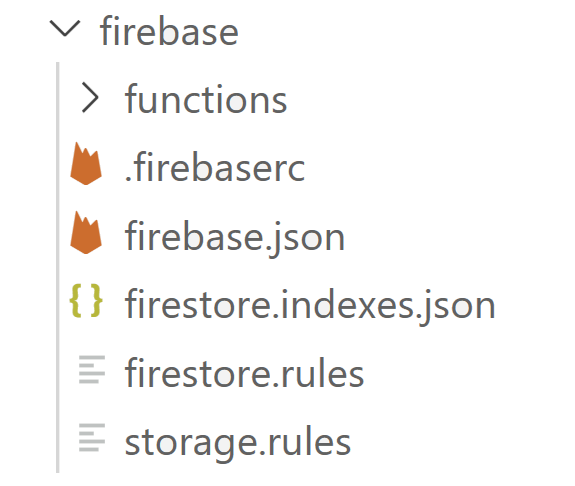
\includegraphics[width=0.6\linewidth]{images/firebase_structure.png}}
  \caption{Schemat struktury projektu Firebase}
  \label{fig:firebase-struktura}
\end{figure}

Pliki \filename{.firebaserc} oraz \filename{firebase.json} są plikami konfiguracyjnymi w formacie JSON. Pierwszy zawiera identyfikator projektu, a drugi konfigurację poszczególnych usług. Ich zawartość po poprawnej inicjalizacji wymagała jedynie delikatnych poprawek.

Katalog \filename{functions} przechowuje kod funkcji Firebase Functions. Jest to zdecydowanie najbardziej obszerna część projektu Firebase i jego zawartość zostanie opisana dokładnie w sekcji \ref{projekt-funkcje}.

Plik \filename{firestore.indexes.json} zawiera indeksy bazy danych Firestore, przechowywane w formacie JSON. Plik ten nie był edytowany manualnie, ze względu na swoją dość skomplikowaną strukturę. Zamiast tego indeksy były tworzone za pomocą wygodnego interfejsu dostępnego przy pomocy przeglądarki internetowej, a następnie wprowadzane do wspomnianego pliku odpowiednią komendą wiersza poleceń. Posiadanie ich bowiem w pliku \filename{firestore.indexes.json} umożliwia stworzenie wszystkich na raz, zamiast mozolnego dodawania przy pomocy przeglądarki. Okaże się to bardzo przydatne w przypadku potrzeby ponownego wdrożenia projektu.

Ostatnie dwa pliki, czyli \filename{firestore.rules} oraz \filename{storage.rules} zawierają reguły bezpieczeństwa Firebase Security Rules, odpowiednio dla bazy Firestore i magazynu plików Cloud Storage. Zostaną one przedyskutowane w sekcji \ref{projekt-reguły}.

\section{Firebase Functions}
\label{projekt-funkcje}

Funkcje są fragmentami kodu, które mogą być wykonywane w odpowiedzi na różne zdarzenia i wywoływać inne usługi. Wykorzystują środowisko Node.js i język TypeScript, a związany z nimi kod, znajdujący się w katalogu \filename{functions} projektu, tworzy typową dla tego środowiska strukturę. To co najważniejsze, czyli kod samych funkcji, umieszczony jest w podkatalogu \filename{src}.

Podczas pisania kodu wykorzystano narzędzie ESlint, które zapewnia jego statyczną analizę w celu wczesnego sygnalizowania błędów. Ponadto ułatwia utrzymanie spójności stosowanych konwencji, takich jak poprzedzanie nieużywanych parametrów znakiem podkreślenia, czy konsekwentne używanie wcięć.

W rozważanym projekcie wykorzystanych zostało 37 funkcji, które można podzielić na cztery kategorie: funkcje wywoływane bezpośrednio, wywoływane okresowo, poprzez modyfikację danych oraz poprzez modyfikację plików. 

\subsection{Funkcje wywoływane bezpośrednio}

Największą część funkcji stanowią te, które są wywoływane bezpośrednio przez aplikacje klienckie. Mogą wówczas zostać przekazane ewentualne argumenty, a w wyniku ich wykonania może zostać zwrócona wartość.

Alternatywę dla tego typu delegowania zadań do funkcji przez aplikacje mobilne stanowi bezpośrednie ich wykonanie po stronie klienckiej. Nie zawsze można jednak na to pozwolić, ponieważ przerwanie niektórych zadań może zostawić system w stanie niespójnym. Środowisko funkcji jest znacznie bezpieczniejsze i stanowi dobre miejsce na wykonywanie takich operacji. 

Ten rodzaj funkcji musiał również zostać wykorzystany do ustawiania przez aplikacje klienckie danych, z których walidacją nie były w stanie poradzić sobie reguły bezpieczeństwa Firebase Security Rules. W celu weryfikacji niektórych informacji konieczne było bowiem wykonanie żądania do API map, co dla reguł nie jest możliwe, a dla funkcji już tak. 

Ostatecznie, aby zachować spójność i nie wykonywać części operacji modyfikacji bezpośrednio w bazie, a części za pośrednictwem funkcji, postanowiono dla wszystkich preferować drugą możliwość. Bezpośrednich modyfikacji dokonywano natomiast jedynie wtedy, gdy było to naprawdę uzasadnione.

Na listingu \ref{lst:function-onCall} została przedstawiona przykładowa, bezpośrednio wywoływana funkcja, która służy do ustawiania obszaru świadczenia usług przez wykonawcę. Wymaga ona podania identyfikatora lokalizacji oraz długości promienia w kilometrach jako argumentów. Zostało to ukryte na listingu w celu jego uproszczenia, lecz korzysta ona z Google Geocoding API, aby sprawdzić poprawność identyfikatora i pobrać nazwę miejsca, a następnie dokonuje aktualizacji odpowiednich wartości w bazie danych.

\begin{minipage}{\linewidth}
\lstinputlisting[
caption=Funkcja wywoływana bezpośrednio, label={lst:function-onCall}
]{listings/function_invoked.ts}
\end{minipage}

Tego typu funkcje posiadają dwa parametry. Pierwszym są dane, które zostały przekazane podczas ich wywołania, a drugi zawiera dodatkowe informacje, z których najczęściej wykorzystywanym jest identyfikator wywołującego ją użytkownika.

W przypadku jawnie wywoływanych funkcji ważna jest walidacja danych, które zostały do nich przekazane. Należało każdorazowo sprawdzić, czy posiadają one odpowiednie typy oraz czy przyjmują odpowiednie wartości. W tym celu została wykorzystana biblioteka Joi, która znacznie ułatwia to zadanie poprzez możliwość definiowania schematów, na podstawie których poprawność parametrów mogła być łatwo oceniana.

Przykładowy schemat przedstawiony na listingu \ref{lst:function-invoke-schema} określa, że przekazane dane muszą zawierać dwie wymagane wartości: \code{placeId} oraz \code{radius}. Pierwsza musi być łańcuchem tekstowym o długości od 1 do 100 znaków, a druga liczbą całkowitą z zakresu pomiędzy 0 oraz \verb|MAX_AREA_RADIUS|. Ograniczenia te zostały wyrażone w czytelny oraz zwarty sposób, w przeciwieństwie do długich, powtarzalnych instrukcji warunkowych, które byłyby konieczne bez biblioteki Joi.

\begin{minipage}{\linewidth}
\lstinputlisting[
caption=Przykładowy schemat biblioteki Joi,
label={lst:function-invoke-schema}
]{listings/function_invoked_schema.ts}
\end{minipage}

\subsection{Funkcje wywoływane okresowo}

Funkcje wywoływane okresowo to takie, których wykonanie odbywa się periodycznie, o ustalonym czasie. Nie mogą być już wywoływane przez aplikacje klienckie, a dzieje się to samoistnie. Wykorzystano ich niewiele, lecz pełnią ważne role.

\begin{minipage}{\linewidth}
\lstinputlisting[
caption=Funkcja wywoływana okresowo,
label={lst:function-scheduled}
]{listings/function_scheduled.ts}
\end{minipage}

Na listingu \ref{lst:function-scheduled} została przedstawiona przykładowa funkcja wywoływana okresowo, która jest odpowiedzialna za zamykanie zleceń, których czas ważności minął. Jest on wyrażany z dokładnością co do dnia, więc wykonywanie jej raz na dobę o północy jest wystarczające. Czas ten jest zapisany w postaci wyrażenia \verb|0 0 * * *|, które wykorzystuje składnię crontab. Zostało ono wyjaśnione na rysunku \ref{fig:crontab}. Składnia ta nie zawsze jest czytelna, lecz daje duże możliwości. Dla każdej funkcji, oprócz wyrażonego w ten sposób czasu, ustalana jest również strefa czasowa na polską. Jest to konieczne, ponieważ domyślną jest strefa czasowa Los Angeles, co powoduje niechciane przesunięcie w czasie wykonywania.

\begin{figure}[ht!]
  \centering
  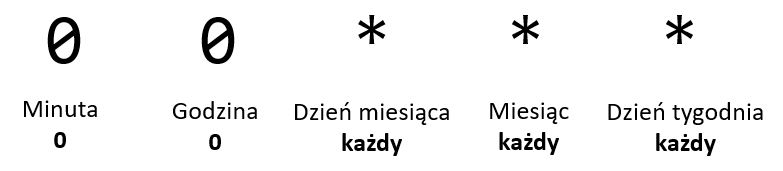
\includegraphics[width=\linewidth]{images/crontab.png}
  \caption{Schemat wyjaśniający wykorzystane wyrażenie crontab}
  \label{fig:crontab}
\end{figure}

\subsection{Funkcje wywoływane modyfikacją danych}

Funkcje wywoływane modyfikacją danych są uruchamiane automatycznie w odpowiedzi na wykonanie określonej operacji w określonej części bazy Firebase Firestore. Mogą być uruchamianie po dodaniu dokumentu, jego usunięciu lub aktualizacji. Nasłuchiwanie tych operacji może być prowadzone dla konkretnych dokumentów lub całych kolekcji.

Głównym zastosowaniem omawianego rodzaju funkcji okazało się utrzymywanie spójności w bazie danych. Pomiędzy znajdującymi się w niej dokumentami istnieją bowiem pewne zależności, które należy egzekwować. Przykładem ich wykorzystania w tym kontekście jest aktualizacja średniej oceny wykonawcy po wykryciu dodania nowej, aktualizująca ostatnio wysłanej wiadomości po nadaniu kolejnej, czy usuwanie komentarzy wykonawcy po wykryciu jego usunięcia.

Poza utrzymywaniem spójności funkcje wywoływane modyfikacją danych okazały się również przydatne do wysyłania powiadomień do użytkowników. Przykładem tego jest nasłuchiwanie utworzenia nowego dokumentu w kolekcji wiadomości, by wysłać komunikat o nowej, nieodczytanej wiadomości do odpowiedniego użytkownika, gdy to nastąpi.

% Brak przecinka przed zamiast
Na listingu \ref{lst:function-firestore} przedstawiona została przykładowa funkcja, której zadanie polega na aktualizacji ostatnio wysłanej wiadomości, gdy zostanie dodana nowa. W tym celu nasłuchuje dodawania dokumentów, których lokalizacja pokrywa się z podaną ścieżką. Zawiera ona w dwóch miejscach nazwy w nawiasach klamrowych, zamiast identyfikatorów dokumentów. Oznaczają one, że dany jej fragment może zostać dopasowany do dowolnego dokumentu. Pierwszy argument z którym wywoływana jest funkcja stanowi zawartość nowo stworzonego dokumentu, a drugi zawiera między innymi identyfikator użytkownika dokonującego modyfikacji oraz fragmenty ścieżki, które zostały dopasowane do wspomnianych wcześniej nazw w nawiasach klamrowych. Dzięki tym argumentom wewnątrz ciała funkcji możliwa jest odpowiednia aktualizacja ostatniej wiadomości.

\begin{minipage}{\linewidth}
\lstinputlisting[
caption=Funkcja wywoływana modyfikacją danych,
label={lst:function-firestore}
]{listings/function_firestore.ts}
\end{minipage}

\subsection{Funkcje wywoływane modyfikacją plików}

Istotny rodzaj wykorzystywanych funkcji stanowią te, które są wywoływane modyfikacją plików przechowywanych w usłudze Firebase Storage. Przede wszystkim możliwe jest wykonywanie ich w odpowiedzi na dodawanie oraz usuwanie plików. Dostępne są również inne zdarzenia, które je uruchamiają, lecz nie zostały użyte.

Rozważane funkcje są wykorzystywane do synchronizacji pomiędzy usługą Firebase Cloud Storage, przechowującą pliki, a bazą danych. Można to rozważyć na przykładzie zdjęć profilowych. Gdy wykonawca ustawia swoje zdjęcie, to jest ono wysyłane przez aplikację kliencką bezpośrednio do Cloud Storage. W tej chwili dodawanie pliku wywołuje wykonanie funkcji, która aktualizuje w bazie danych informacje dotyczące zdjęcia profilowego, czyli jego adres URL oraz datę zmiany. Podobnie, gdy wykonawca usuwa zdjęcie, to aplikacja kliencka usuwa je bezpośrednio z usługi magazynu plików. Jest to następnie wykrywane przez funkcję, która odpowiednio aktualizuję dane wewnątrz Firestore.

Na listingu \ref{lst:function-storage} została przedstawiona funkcja, która aktualizuje bazę danych po usunięciu zdjęcia profilowego. Jest ona w rzeczywistości wykonywana po usunięciu każdego pliku i nie ma możliwości zawężenia nasłuchiwanego przez nią obszaru jedynie do katalogu zdjęć profilowych. Parametr z którym jest wywoływana umożliwia jednak uzyskanie ścieżki do pliku, który spowodował jej wykonanie i na tej podstawie można stwierdzić, czy rzeczywiście jest to zdjęcie profilowe.

\begin{minipage}{\linewidth}
\lstinputlisting[
caption=Funkcja wywoływana modyfikacją plików,
label={lst:function-storage}
]{listings/function_storage.ts}
\end{minipage}

Wewnątrz funkcji wywoływanych modyfikacją plików nie jest możliwe uzyskanie identyfikatora użytkownika, który dokonał zmiany. Fakt ten okazał się dla autora dość zaskakujący, ponieważ wydaje się to być jedną z podstawowych informacji, a funkcje wywoływane modyfikacją bazy Firestore z jakichś powodów już ją udostępniają, co wydaje się niekonsekwentne. Obejściem tego problemu okazało się stworzenie katalogów o nazwach odpowiadających identyfikatorom użytkowników, a następnie ograniczenie im dostępu za pomocą Firebase Security Rules jedynie do swoich folderów. Dzięki temu analizując ścieżkę zmodyfikowanego pliku można było uzyskać informację o użytkowniku, który tego dokonał.

\section{Firebase Security Rules}
\label{projekt-reguły}

Firebase Security Rules to reguły, które pozwalają na ograniczenie aplikacjom klienckim dostępu do danych przechowywanych przez Firebase. Usługami dla których określono reguły są Firestore oraz Cloud Storage. Było to konieczne, aby zapewnić bezpieczeństwo dla bazy danych oraz magazynu plików.

Pozornie określanie reguł bezpieczeństwa może wydawać się niepotrzebne, ponieważ już sama logika aplikacji klienckich została zaprojektowana w taki sposób, aby uniemożliwić niechciane scenariusze. Nie jest to jednak wystarczające, ponieważ należy mieć na uwadze możliwość ingerencji w aplikacje niepożądanych osób lub zdobycia przez nie w inny sposób dostępu, w celu uzyskania pewnych korzyści, kradzieży danych czy spowodowania awarii aplikacji. Poza tym zawsze istnieje możliwość popełnienia błędów w logice aplikacji przez programistę, a kolejna warstwa zabezpieczeń, w postaci Firebase Security Rules, pozwala zablokować te operacje, które nie powinny mieć miejsca.

Stworzone reguły mają zastosowanie jedynie do aplikacji klienckich. W żaden sposób nie wpływają one na operacje, które mogą być wykonywane w ramach Firebase Functions. Dzieje się tak, ponieważ środowisko, w którym funkcje są wykonywane, jest uważane za środowisko w pełni kontrolowane, a więc bezpieczne.  

\subsection{Reguły dla Firebase Firestore}

Reguły bezpieczeństwa dla Firestore działają na poziomie dokumentów i umożliwiają określenie osobnych uprawnień dla operacji odczytu oraz zapisu. Jeżeli potrzebny jest większy poziom szczegółowości uprawnień to zapis może zostać rozbity na uprawnienia do tworzenia, aktualizacji oraz usuwania. Najważniejsze wprowadzone reguły są następujące:

\begin{itemize}
    \item Dla kolekcji zawierających usługi oraz kategorie usług uniemożliwiono zapis, ponieważ zawierają wartości, których zmian nie przewidziano.
    \item Dla kolekcji matchings, która stanowi jedynie szczegół implementacyjny, zarówno zapis, jak i odczyt został zablokowany.
    \item Na odczyt wiadomości zezwolono jedynie użytkownikowi będącemu jego nadawcą lub odbiorcą.
    \item Na odczyt oferty zezwolono jedynie wykonawcy, który ją złożył oraz klientowi, któremu została złożona.
\end{itemize}

% TODO: Można wspomnieć o braku możliwości stworzenia ograniczenia na joby

Ograniczeniem, które okazało się problemem, jest to, że można uniemożliwić odczyt jedynie dla całych dokumentów, a nie można tego zrobić na poziomie poszczególnych ich pól. W związku z tym nie udało się zablokować odczytu tych, które stanowią jedynie szczegóły implementacyjne. Przykładem takich pól są dwa znajdujące się w dokumentach wykonawców, przechowujące sumę oraz liczbę ocen. Są wykorzystywane jedynie w celu wyliczenia średniej oceny i nie są używane przez aplikacje klienckie, a pomimo tego będą one miały do nich dostęp.

Rozwiązaniem problemu pól będących szczegółami implementacyjnymi mogłoby być przeniesienie ich do osobnych dokumentów oraz kolekcji, dla których dostęp mógłby zostać już ograniczony. Takie podejście rozwiązałoby go, lecz wiązałoby się z powstaniem dużej liczby dodatkowych kolekcji, zwiększających stopień komplikacji projektu. Biorąc pod uwagę, że rozważane pola nie przechowują żadnych krytycznych danych i ich udostępnienie nie powinno stanowić zagrożenia bezpieczeństwa ani prywatności, zdecydowano się to zaakceptować.

\subsection{Reguły dla Firebase Cloud Storage}

Reguły wykorzystywane przez Firebase Cloud Storage działają na poziomie plików i umożliwiają określanie osobnych zasad dla ich odczytu i zapisu. Gdy nie jest to wystarczające, to zapis można doprecyzować przy pomocy reguł tworzenia, aktualizacji i usuwania.

Przez usługę przechowywane są jedynie dwa typy danych: zdjęcia profilowe oraz obrazy wysyłane przez chat. Z tego powodu liczba reguł wymagana przez nią okazała się znacznie mniejsza niż w przypadku Firestore. 

Stworzone reguły ograniczają możliwość dodawania plików jedynie do przeznaczonych dla tego celu katalogów. Określają, że w przypadku zdjęć profilowych możliwe są wszystkie operacje zapisu, ponieważ wykonawcy mogą dodawać, aktualizować oraz usuwać swoje zdjęcia. Dodatkowo wymagają, aby nazwy plików przesyłanych do katalogu zdjęć profilowych stanowiły identyfikatory użytkowników połączone z rozszerzeniem png. Jeżeli któreś z wymagań nie będzie spełnione, to operacja zostanie odrzucona.
W przypadku zdjęć wysyłanych przez chat, poza koniecznością umieszczenia ich w odpowiednim katalogu, wymagane jest posiadanie przez nie rozszerzenia png. Ponadto możliwe operacje są ograniczone jedynie do tworzenia nowego pliku, ponieważ nie przewidziano możliwości aktualizowania, ani usuwania już wysłanego przez chat zdjęcia
